\documentclass[aspectratio=169]{slide-en}

\usepackage{physics}
\usepackage{caption}
\usepackage{subcaption}

\usepackage{scrextend}

\usepackage{algorithm}
\usepackage{algpseudocodex}
\usepackage{amsmath}
\usepackage{array}
\usepackage{bbm}
\usepackage{csvsimple} % csvreader

\graphicspath{{src/}{src/rlime-paper/src/}}
\addbibresource{src/rlime-paper/src/ref.bib}

\newcommand{\ispace}{\mathbb{D}^{m}}
\newcommand{\Prec}{\operatorname{acc}}
\newcommand{\Cov}{\operatorname{cov}}
\newcommand{\cands}{\bar{\mathcal{A}}}
\algnewcommand{\IIf}[1]{\State\algorithmicif\ #1\ \algorithmicthen\ }
\renewcommand{\algorithmicrequire}{\textbf{Input:}}
\renewcommand{\algorithmicensure}{\textbf{Output:}}


\newcommand{\dtrain}{D_{\mathrm{train}}}
\newcommand{\dtest}{D_{\mathrm{test}}}
\newcommand{\dmis}{D_{\mathrm{mis}}}
\newcommand{\dchange}{D_{\mathrm{change}}}

\title{\texorpdfstring{
  R-LIME:\@ Rectangular Constraints and Optimization
  for Local Interpretable Model-agnostic Explanation Methods
}{}}
\author{Genji Ohara, Keigo Kimura and Mineichi Kudo}
\date{December 2024}
\institute{%
  Division of Computer Science and Information Technology \\
  Graduate School of Information Sci.\@ and Tech., Hokkaido University \\
  Sapporo 060--0814, JAPAN
}

\begin{document}

\section*{Background}
\begin{frame}{}
  \colorrect{red!30}{Interpretable Machine Learning}
  \bigskip
  \begin{columns}[]
    \begin{column}{0.4\textwidth}
      \begin{itemize}
        \item Simple ML models (White-box)
              \begin{itemize}
                \item Linear Models
                \item Decision Trees
              \end{itemize}
              \smallskip
              \textrightarrow{} Decision process is \underline{clear}
      \end{itemize}
      \centering
      \COLabel{simple}{}
    \end{column}
    \begin{column}{0.44\textwidth}
      \begin{itemize}
        \item Complex ML models (Black-box)
              \begin{itemize}
                \item Deep Neural Networks
                \item Ensemble Models
              \end{itemize}
              \smallskip
              \textrightarrow{} Decision process is \underline{unclear}
      \end{itemize}
      \centering
      \COLabel{complex}{}
    \end{column}
  \end{columns}
  \begin{tikzpicture}[remember picture,overlay]
    \draw (simple) edge [->, thick, bend right=20] node [midway, below]
      {\colorrect{blue!30}{Approximate Locally}} (complex);
  \end{tikzpicture}
\end{frame}

\section{Related Work: LIME \& Anchor}

\begin{frame}{}
  \vspace{1.5em}
  \begin{columns}[t]
    \begin{column}{0.45\textwidth}
      LIME%\footnote[frame]{\fullcite{ribeiro2016why}}
      \begin{itemize}
        \item Approximate the model locally based on the perturbed samples
      \end{itemize}
      \begin{figure}
        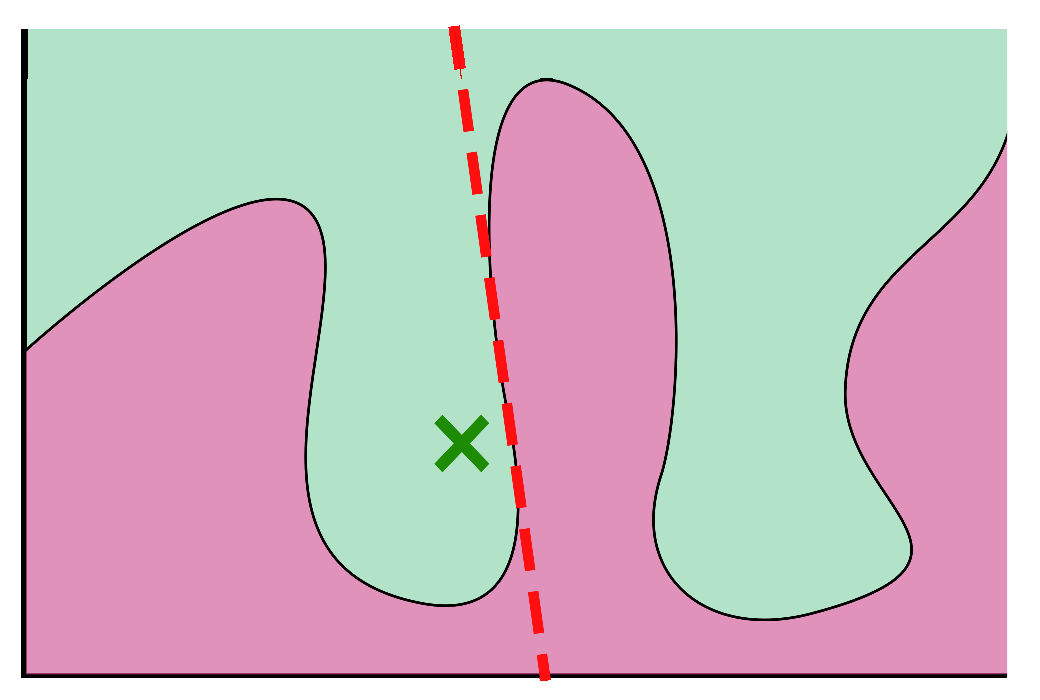
\includegraphics[scale=.25]{img/visual-lime}
        \caption{Visual illustration of LIME\@.}
      \end{figure}
      \textbf{But how general is this explanation?}
    \end{column}
    \begin{column}{0.55\textwidth}
      Anchor
      \begin{itemize}
        \item Maximize the rectangular region as long as
              the model's outputs are mostly consistent.
      \end{itemize}
      \begin{figure}
        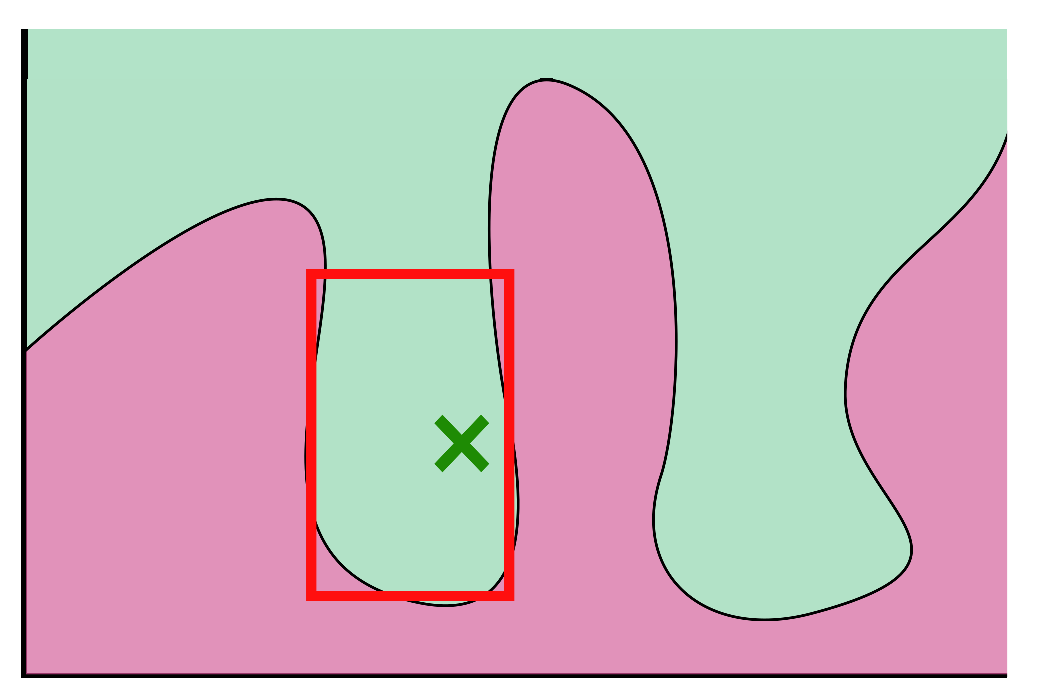
\includegraphics[scale=.25]{img/visual-anchor}
        \caption{Visual illustration of Anchor.}
      \end{figure}
      \textbf{But how much influence does each feature have?}
    \end{column}
  \end{columns}
\end{frame}

\section{Proposed Method: R-LIME}

\begin{frame}{}
  \begin{columns}[]
    \begin{column}{0.55\textwidth}
      \colorrect{red!20}{\textbf{R-LIME (Ruled LIME)} = LIME + Anchor}

      \bigskip
      \begin{itemize}
        \item Approximate in rectangular region
        \item Maximize the rectangular region as long as
              the approximation is accurate.
        \item Express the region as a conjunction of feature predicates \\
              \smallskip
              \footnotesize{
                ex. $\textrm{Gender} = \textrm{'Male' AND } 20\le\textrm{Age} < 30$
              }
      \end{itemize}
    \end{column}
    \begin{column}{0.40\textwidth}
      \begin{figure}
        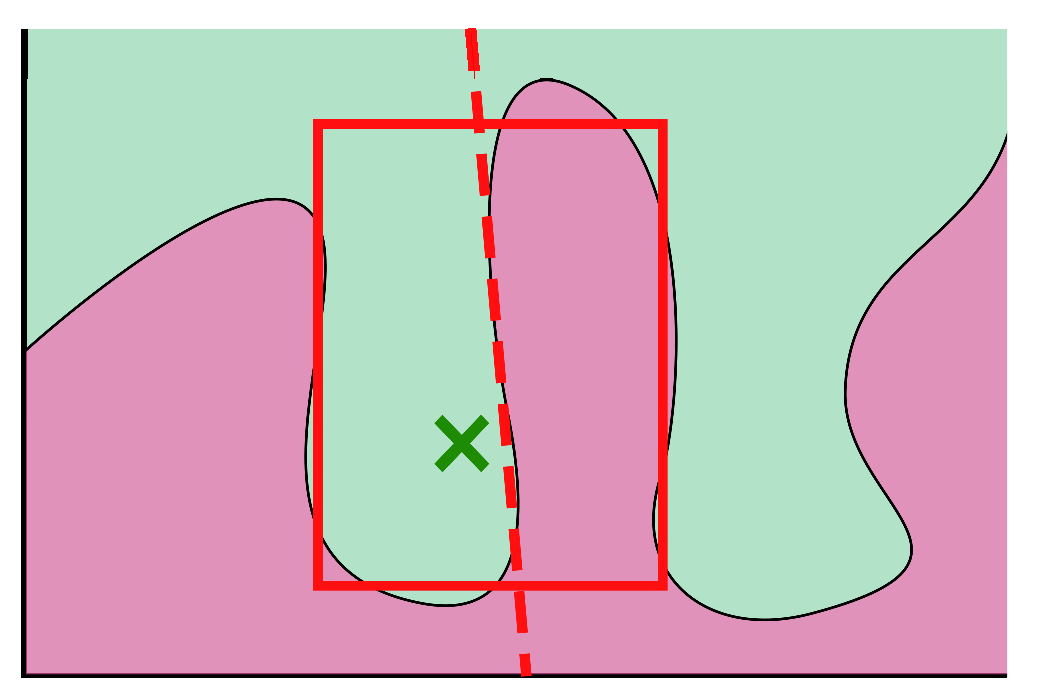
\includegraphics[width=\textwidth]{img/visual-rlime3}
      \end{figure}
    \end{column}
  \end{columns}
\end{frame}

\section{Experiments}

\begin{frame}{}
  \vspace{-1.5em}
  \begin{columns}[t]
    \begin{column}{0.48\textwidth}
      \begin{figure}
        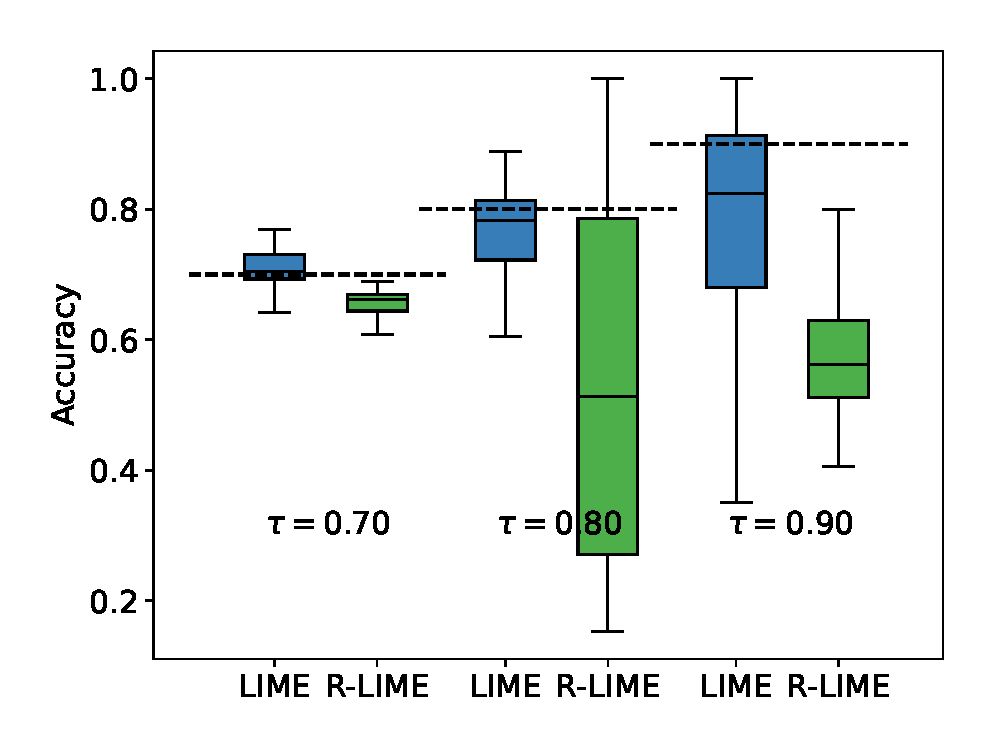
\includegraphics[height=142pt]{experiments/exp2/box_plot}
      \end{figure}
      \begin{itemize}
        \item Much higher accuracy of R-LIME than LIME, especially for large $\tau$
      \end{itemize}
    \end{column}
    \begin{column}{0.48\textwidth}
      \begin{figure}
        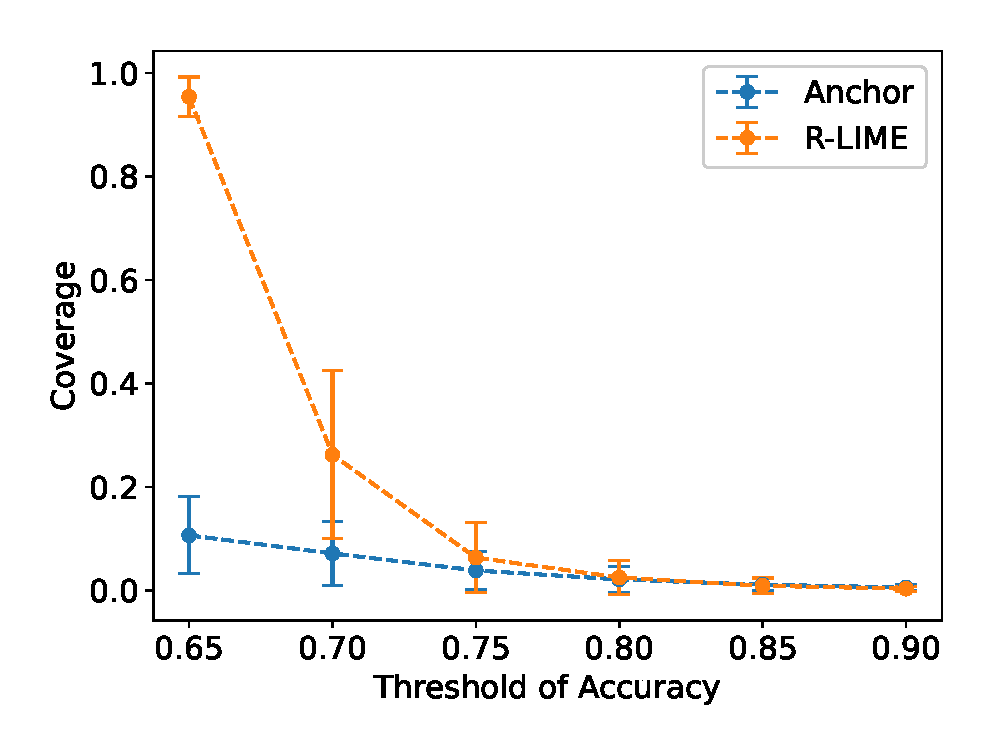
\includegraphics[height=140pt]{experiments/exp2/comp_cov}
      \end{figure}
      \begin{itemize}
        \item Much higher coverage of R-LIME than Anchor, especially for small $\tau$
      \end{itemize}
    \end{column}
  \end{columns}
\end{frame}

\section{Conclusion}

\begin{frame}{}
  \renewcommand{\arraystretch}{1.5}
  \tabcolsep=1.5em
  \begin{center}
    \begin{tabular}{cccc}
                          & LIME         & Anchor       & \textbf{R-LIME} \\
      \midrule
      Feature Importance  & \checkmark{} & $\times$     & \checkmark{}    \\
      Optimal Scope       & $\times$     & \checkmark{} & \checkmark{}    \\
      Interpretable Scope & $\times$     & \checkmark{} & \checkmark{}    \\
    \end{tabular}
  \end{center}
  \bigskip
  \hspace{0.05\textwidth}
  \setbeamercolor{myblue}{bg=blue!15}
  \begin{beamercolorbox}[wd=0.85\textwidth,rounded=true]{myblue}
    Our methods achieves interpretability of both explanation and its scope!

    \smallskip
    \begin{addmargin}[1em]{2em}
      Also:
      \begin{itemize}
        \item More accurate than LIME
        \item More general than Anchor
      \end{itemize}
    \end{addmargin}
  \end{beamercolorbox}
\end{frame}

\end{document}
